\documentclass{article}
\usepackage{colortbl}
\usepackage{tikz}
\usepackage{multicol}
\usepackage{xcolor}
\usepackage{ifthen}
\usepackage{array}

% Színek definiálása
\definecolor{grayrow}{gray}{0.9}  % Szürke háttérszín
\definecolor{lightblue}{rgb}{0.8, 0.85, 1}  % Világoskék háttérszín

% Váltakozó háttérszínű táblázathoz
\newcolumntype{A}{>{\columncolor{grayrow}}c}  % Szürke sor
\newcolumntype{B}{c}  % Fehér sor
\newcolumntype{C}{>{\columncolor{lightblue}}c}  % Világoskék sor

% Számláló a kulcsgondolatok számára
\newcounter{gondolat}
\setcounter{gondolat}{0}

% Saját környezet kulcsgondolatokhoz
\newenvironment{kulcsgondolat}[1][Kulcsgondolatok]{
    \noindent\rule{\textwidth}{0.4pt} \\  % Vízszintes vonal
    \textbf{\centering #1} \par  % Cím középre zárva
    \noindent\rule{\textwidth}{0.4pt} \\  % Vízszintes vonal
    \begin{center}
    \begin{minipage}{0.8\textwidth}  % 80%-os szélesség
    \setlength{\parindent}{0pt}  % Behúzás nélküli új bekezdés
}{
    \end{minipage}
    \end{center}
    \noindent\rule{\textwidth}{0.4pt}  % Vízszintes vonal
}

% Helyi parancs a kulcsgondolatok kiírására
\newcommand{\gondolat}[1]{%
    \stepcounter{gondolat}%
    \noindent\makebox[3em][l]{\thegondolat} #1 \par
}


\begin{document}

% 1. Táblázat
\section*{Példák}

\subsection*{1. táblázat. Táblázatok váltakozó szövegszínnel}

\subsubsection*{(a) Háttérszín is váltakozik}
\begin{table}[h!]
\centering
\begin{tabular}{|A|B|C|}
\hline
a & b & c \\
a & b & c \\
a & b & c \\
a & b & c \\
a & b & c \\
\hline
\end{tabular}
\end{table}

\subsubsection*{(b) Csak szövegszín váltakozik}
\begin{table}[h!]
\centering
\begin{tabular}{|c|c|c|}
\hline
\color{red} a & \color{blue} b & \color{orange} c \\
\color{green} a & \color{purple} b & \color{cyan} c \\
\color{magenta} a & \color{teal} b & \color{brown} c \\
\color{olive} a & \color{violet} b & \color{lime} c \\
\color{pink} a & \color{gray} b & \color{yellow} c \\
\hline
\end{tabular}
\end{table}

% 1. ábra
\subsection*{1. ábra. Egységkörök középpontok koordinátái a körökbe írva}
\begin{center}
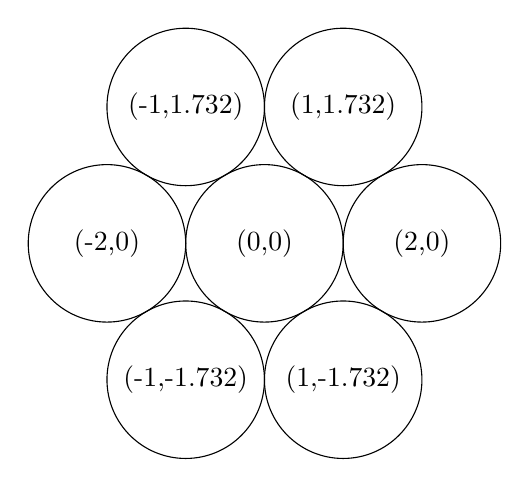
\begin{tikzpicture}
    % Középső vízszintes sor
    \foreach \x/\y in {-2/0, 0/0, 2/0} {
        \draw (\x,\y) circle (1cm);
        \node at (\x,\y) {(\x,\y)};
    }
    
    % Felső sor
    \foreach \x/\y in {-1/1.732, 1/1.732} {
        \draw (\x,\y) circle (1cm);
        \node at (\x,\y) {(\x,\y)};
    }
    
    % Alsó sor
    \foreach \x/\y in {-1/-1.732, 1/-1.732} {
        \draw (\x,\y) circle (1cm);
        \node at (\x,\y) {(\x,\y)};
    }
\end{tikzpicture}
\end{center}

% 1.1. Cikk-cakk
\newpage
\subsection*{1.1. Cikk-cakk}
\def\modulo#1#2{(#1-(#1/#2)*#2)}    % a mod n = a-(a/n)*n   where / is integer division

\newcount\X
\X=1
 \begin{multicols}{3} % Három oszlopos elrendezés
\loop
    \ifnum \numexpr\modulo{\X}{15} = 0
        \the\X \, cikkcakk
    \else
        \ifnum \numexpr\modulo{\X}{3} = 0
            \the\X \, cikk
        \else
            \ifnum \numexpr\modulo{\X}{5} = 0
               \the\X \, cakk
            \else
                \the\X
            \fi
        \fi
    \fi
    \endgraf
    \advance \X by 1
    \unless \ifnum \X>60
    \repeat
    \end{multicols}

% 2. Feladat: Kulcsgondolatok
\section*{Kulcsgondolatok}
\begin{kulcsgondolat}[Fontos gondolatok]
\gondolat{Ez egy kulcsgondolat a dokumentumban.}
\gondolat{Itt van még egy fontos gondolat.}
\gondolat{Ne felejtsük el ezt a kulcsfontosságú információt.}
\end{kulcsgondolat}

% 3. Feladat: Zebra táblázat
\subsection*{Zebra táblázat}
\begin{table}[h!]
\centering
\begin{tabular}{|A|B|C|}
\hline
\rowcolor{grayrow}
1 & 2 & 3 \\
\rowcolor{white}
4 & 5 & 6 \\
\rowcolor{grayrow}
7 & 8 & 9 \\
\rowcolor{white}
10 & 11 & 12 \\
\hline
\end{tabular}
\caption{Zebra táblázat váltakozó háttérszínekkel.}
\end{table}

\end{document}
